\documentclass{article}
\usepackage[T1]{fontenc}
\usepackage[utf8]{inputenc}
\usepackage{polski}
\usepackage{graphicx}
\frenchspacing
\author{
  Emil Kowalczyk\\
  \texttt{230178}
  \and
  Joanna Ściebura\\
  \texttt{204169}
  \and
  Marcel Młodziński\\
  \texttt{217119}
  \and
  Maciek Blankenburg\\
  \texttt{233348}
  \and
}
\title{ Pracownia Problemowa I \\
  \large Odtworzenie algorytmu Eclat na dużym zbiorze danych }
\date{\today}
\usepackage{graphicx}
\setcounter{secnumdepth}{1}
\usepackage{enumitem} %do tworzenia listy ze zdefiniowanym punktorem
\usepackage{float} %do odpowiedniego umieszczania obrazkóW w dokumencie

%komendy do odpowiedniego numerowania obrazów
\usepackage{chngcntr} 
\counterwithin{figure}{section}                           

% zmiana podpisu rysunków
\renewcommand{\figurename}{Rys.}


\begin{document}
	
    \maketitle	
    \clearpage
   
    \tableofcontents
    \clearpage
    
	\section{Wstęp}
		Niniejsza praca omawia zagadnienie wydajności jednego z algorytmów „Data Minningu”, służącego do wydobywania danych za pomocą baz danych. Wykorzystywany w analizie koszykowej, czyli metodzie, która dla tworzy dla zbioru danych zestaw opisujących go przybliżonych reguł asocjacyjnych, tj. powiazań i skojarzeń pomiędzy konkretnymi wartościami zmiennych. Metody asocjacyjne są bardzo przydatne przy operowaniu na dużych zbiorach danych, gdyż przetwarzają one dane w taki sposób, żeby móc wyciągnąć jak najwięcej relacji, które w dziedzinach takich jak sklepy są bardzo przydatne. Przykładowo, pomagają one w ustawianiu produktów tak, żeby klient przy zakupie produktu „X”, zauważył powiązany produkt „Y” i przy okazji go zakupił.   
		
	\section{Organizacja pracy}
		W celu jak najlepszego zorganizowania pracy, korzystaliśmy z wielu narzędzi, które na co dzień użytkowane są w branży „IT” i w przypadku ich potencjalnego braku, wiele współczesnych firm mogło czuć się w swoich działaniach „jak bez jednej ręki”. 	
		
		\subsection{Slack}
		
	Slack traktowany był przez nas jako główny kanał komunikacyjny, jest to darmowa usługa oparta na chmurze, która dzięki posiadaniu wielu narzędzi i usług, używana jest przez największe korporacje informatyczne w naszym kraju. Dzięki możliwości podpinania wielu zewnętrznych aplikacji oraz dzięki funkcjom takim jak „Thread”, zapewnia ona poprawienie organizacji pracy pomiędzy grupą. 

Poniżej widnieje zrzut ekranu z panelu głównego aplikacji:
 		
		\begin{figure}[!h]
			\centering
			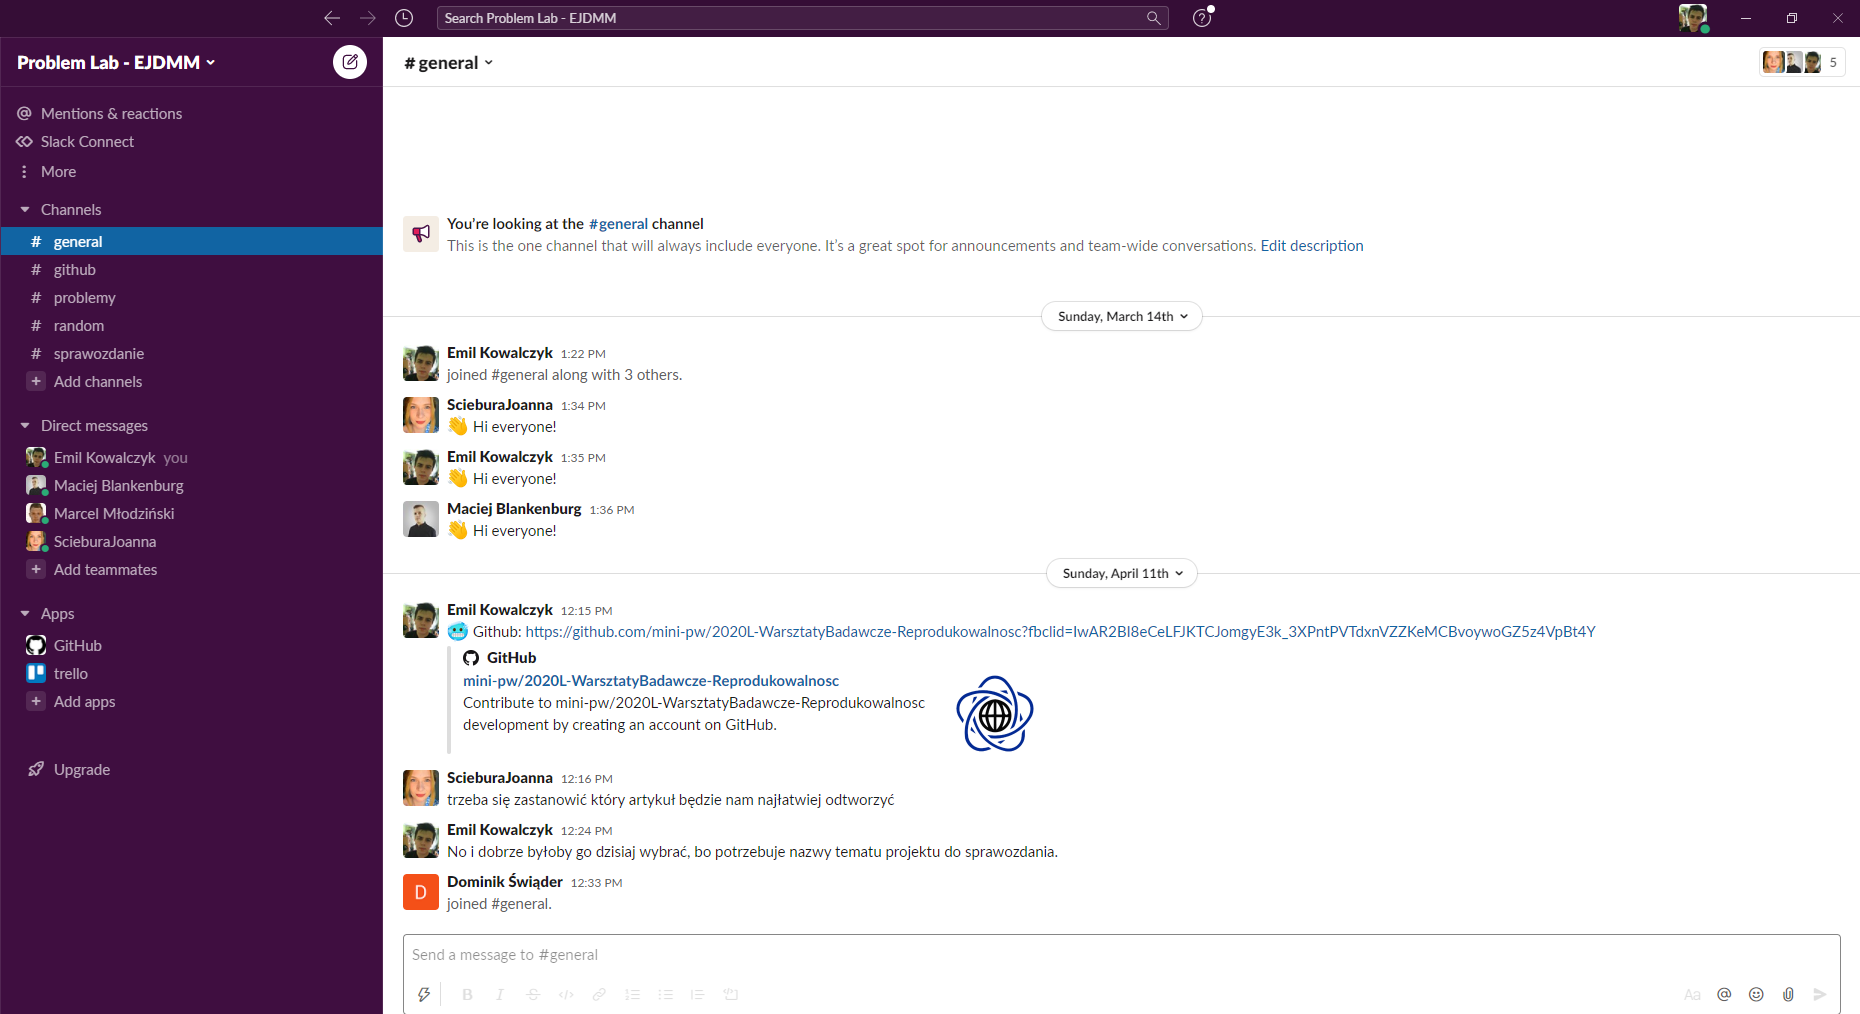
\includegraphics[scale=0.23]{Slack.png}
			\caption{Zrzut ekranu z aplikacji Slack}
		\end{figure}
		
		\begin{figure}[!h]
			\centering
			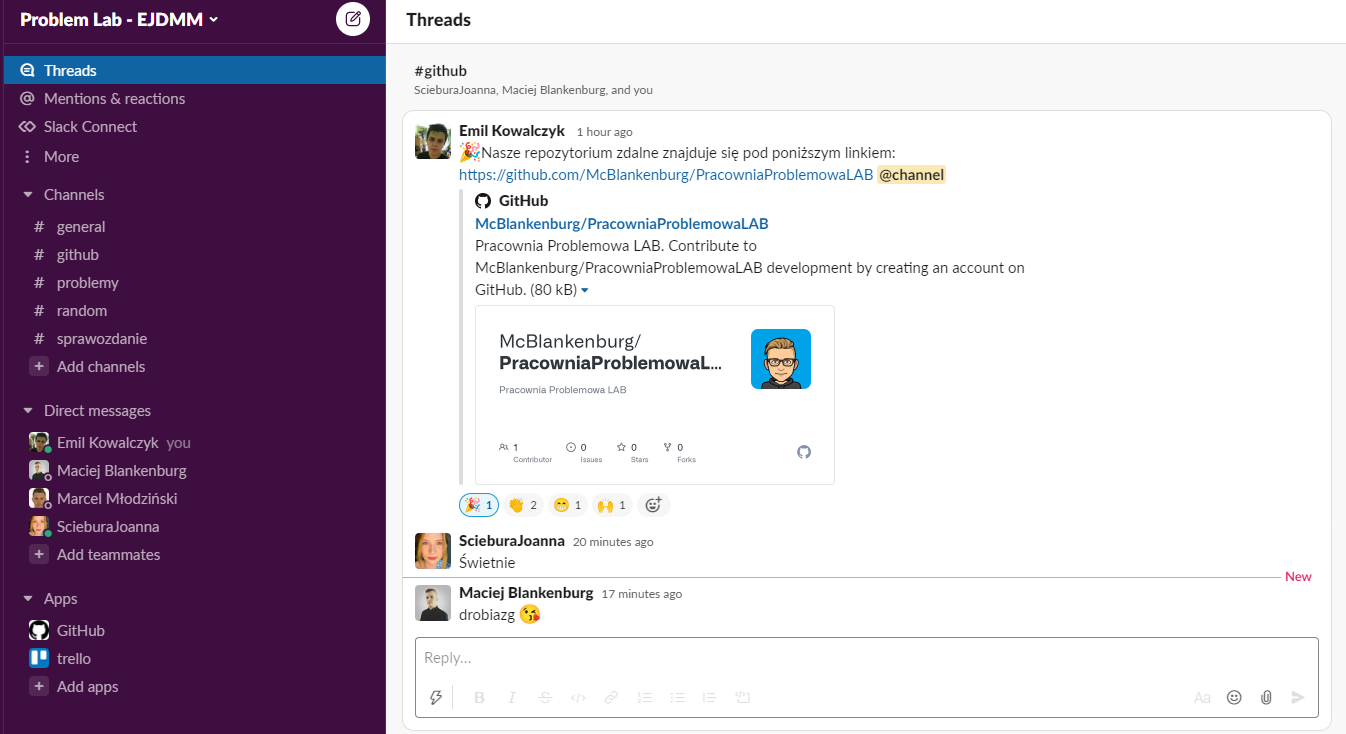
\includegraphics[scale=0.35]{Thread.png}
			\caption{Zrzut ekranu z aplikacji Slack przedstawiający komunikację zespołu}
		\end{figure}
		
Dzięki wyżej wspomnianym funkcjom Slacka, mogliśmy skonfigurować aplikację tak, żeby ta, mogła korzystać z zewnętrznych aplikacji takich jak Trello czy Github, które będą opisane niżej. 

Funkcjonalności podpięcia zewnętrznych aplikacji, umożliwiały śledzenie tego, co dzieje się na zewnętrznych aplikacjach, jednocześnie nie musząc do nich wchodzić. 

		\begin{figure}[!h]
			\centering
			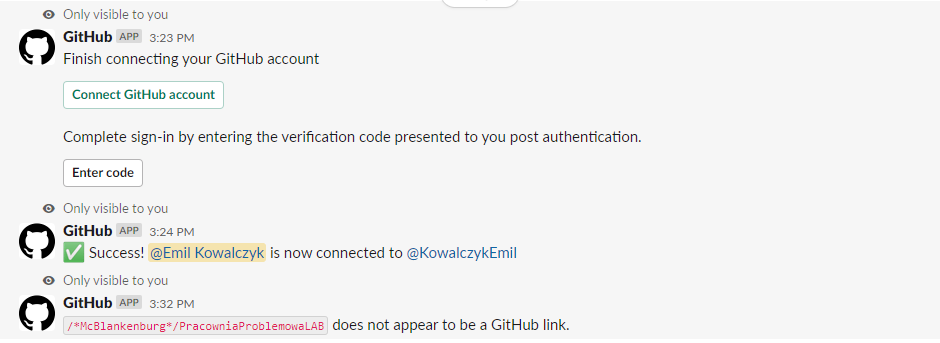
\includegraphics[scale=0.45]{Github.png}
			\caption{Zrzut ekranu z konfiguracji Slacka z Githubem}
		\end{figure}

		
		\subsection{Trello}

		\textbf{Trello} to aplikacja, która pomogła nam w zarządzaniu jednostkami w zespole, jest to internetowa aplikacja do tworzenia list w stylu Kanban. Dzięki niej mogliśmy stworzyć tablicę, na której rozpisane były cele jak i obowiązki każdego z nas. 
		
		\begin{figure}[!h]
			\centering
			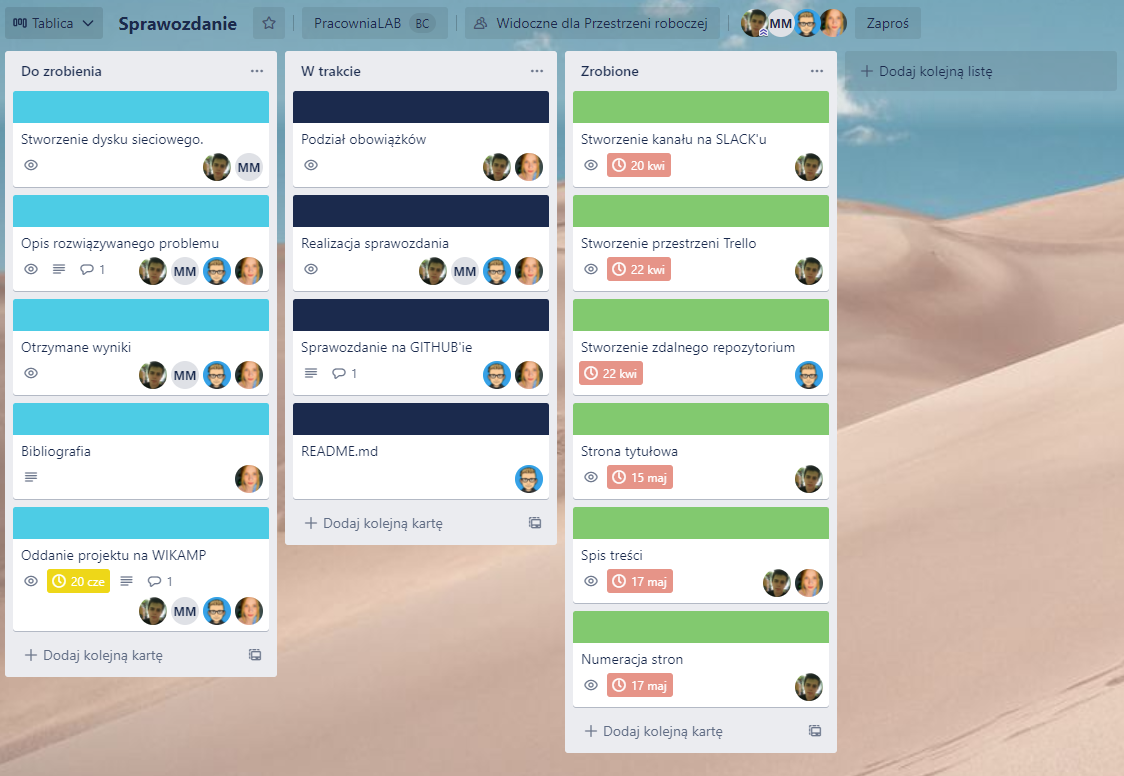
\includegraphics[scale=0.45]{Trello.png}
			\caption{Zrzut ekranu z aplikacji Trello}
		\end{figure}
		
		\subsection{Github}
\textbf{Github} – To nieodłączny element pracy w grupie, czyli hostingowy serwis internetowy, przeznaczony do przechowywania projektów, wykorzystujących system kontroli wersji GIT. 

To właśnie na Githubie, przechowywaliśmy dokumentacje, którą bez problemu każdy z nas mógł sobie pobierać i wprowadzać swoje zmiany w czasie rzeczywistym, tak, że przy poprawnym korzystaniu z systemu kontroli wersji, każdy mógł pracować na świeżo zaktualizowanej pracy, zachowując przy tym całą historię dokumentacji. 

Poniżej widać, że użytkowanie GIT’a, w połączeniu ze zdalnym repozytorium, to naprawdę prosta rzecz i żeby móc bez problemu korzystać z takiej konfiguracji, wystarczy do tego obsługa kilku komend. Dlatego jest to tak popularna rzecz w obecnych czasach. 

		\begin{figure}[!h]
			\centering
			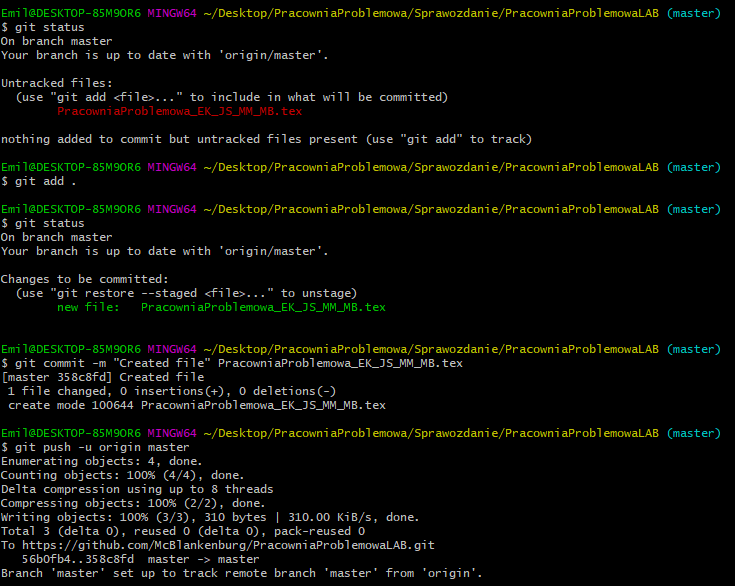
\includegraphics[scale=0.6]{Git.png}
			\caption{Zrzut ekranu z konsoli GIT’a}
		\end{figure}
		
		
		Dzięki wyżej wspomnianemu githubowi, mogliśmy umieszczać zmiany w dokumentacji, w taki sposób, że każda osoba z grupy, niezależnie od tego gdzie się znajdowała, mogła te zmiany widzieć oraz z nich korzystać pobierając sobie obecną wersję projektu np.: dzięki korzystania z funkcji \textbf{git pull}.
		\begin{figure}[!h]
			\centering
			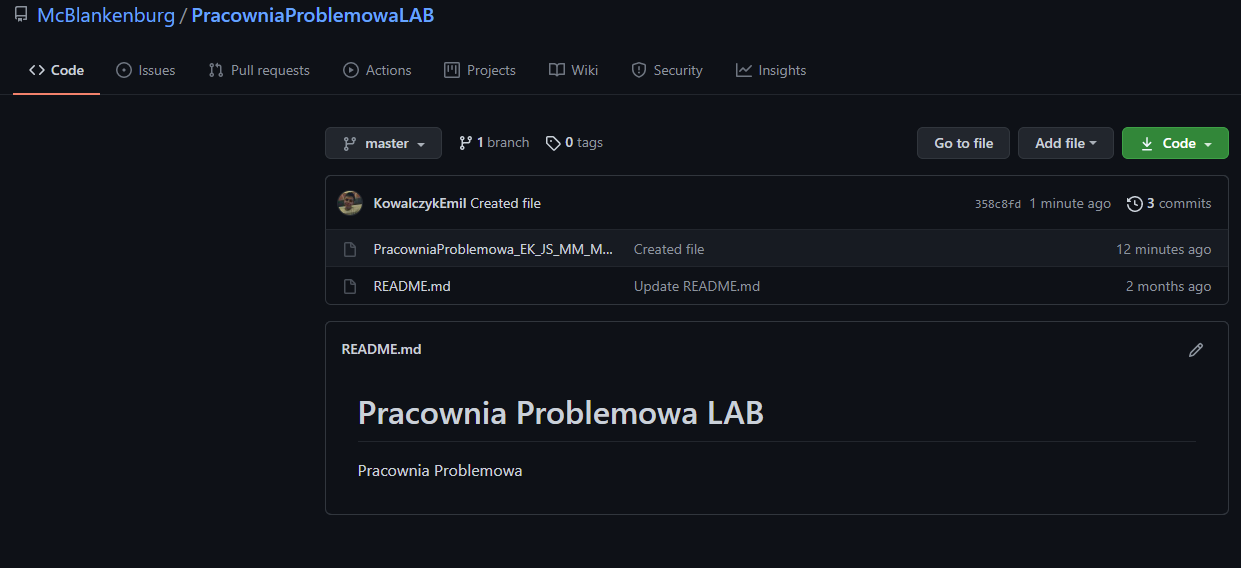
\includegraphics[scale=0.4]{Git2.png}
			\caption{Zrzut ekranu ze zdalnego repozytorium}
		\end{figure}
		
		\subsection{Dropbox}
\textbf{Dropbox} – usługa pozwalała nam przechowywać pliki w przestrzeni chmurowej. Była przez nas rzadko wykorzystywana, jednak wszelakie zrzuty ekranu, były umieszczane właśnie tam, dzięki czemu nasze dyski na lokalnych komputerach, nie muszą przechowywać zbędnych danych, które mogą być przechowywane w chmurze, dodatkowo mając dodatkową funkcjonalność w postaci możliwości pobierania tych danych przez każdą osobę z zespołu w dowolnym momencie.

		\begin{figure}[!h]
			\centering
			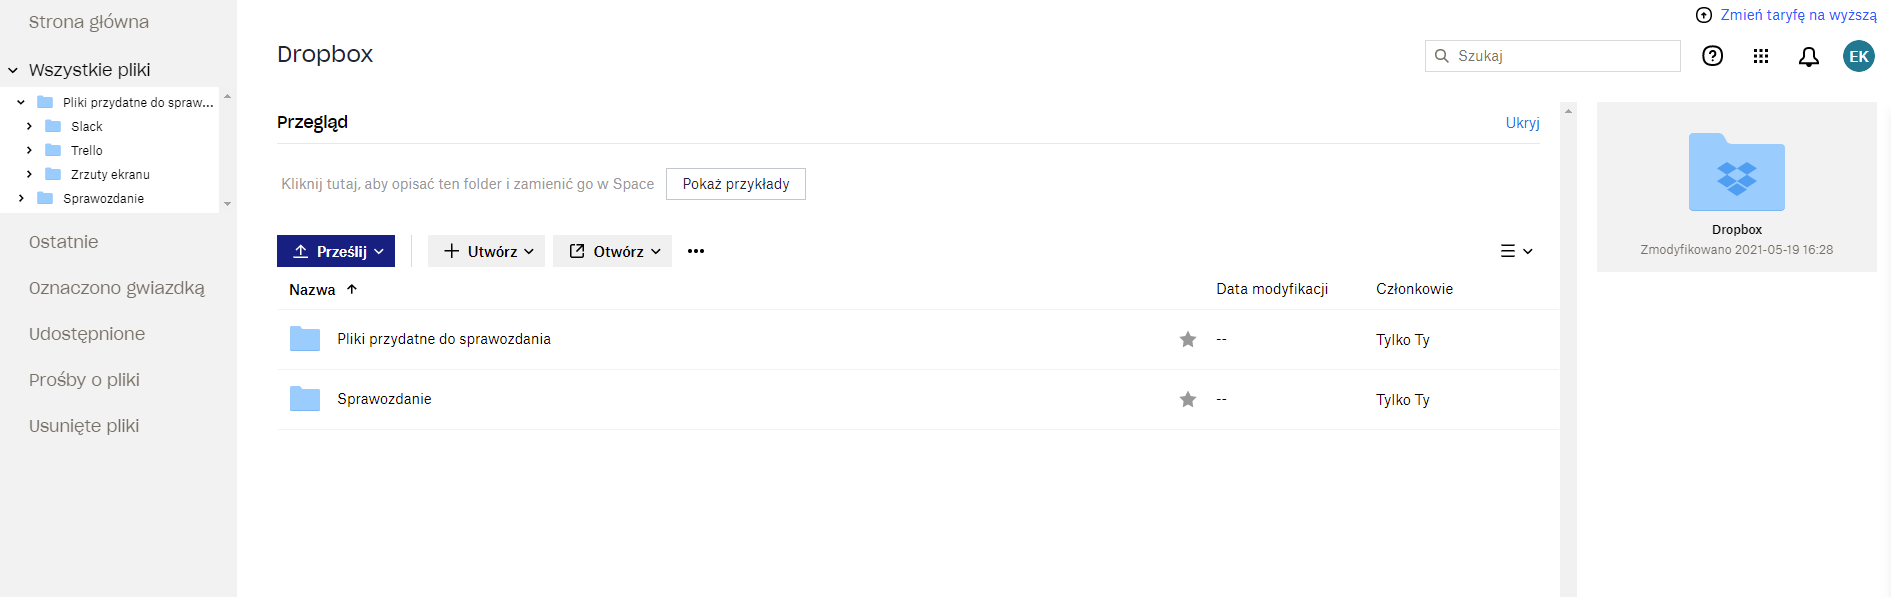
\includegraphics[scale=0.25]{Dropbox.png}
			\caption{Zrzut ekranu z aplikacji dropbox}
		\end{figure}
		
	\newpage
	
	\section{Opis działania algorytmu}

\textbf{Eclat} – jest to algorytm do znajdowania częstych zestawów produktów w transakcji lub bazie danych. Jest to jedna z najlepszych metod uczenia się reguł asocjacyjnych. Algorytm ten, jest używany do generowania częstych zestawów przedmiotów w bazie danych. 

W porównaniu do algorytmu Apriori, w metodzie zaproponowanej przez Zakie’go nastąpiła znacząca redukcja narzutu związanego z operacjami wejścia/wyjścia. Eclat wykonuje trzy odczyty z bazy danych, natomiast algorytmy z rodziny Aprioori muszą przeszukiwać dbazę danych tyle razy, ile wynosi maksymalna długość zbioru częstego. Ponadto, już na początku wykonywania algorytmu Eclat uzyskujemy niezależność pomiędzy procesami. Dzięki czemu nie jest potrzebna synchronizacja w trakcie generacji kolejnych kandydatów na zbiory częste. Algorytm Eclat posiada również istotne wady, główne narzuty związane z komunikacją wynikają z potrzeby ustalenia globalnych tid-list na początku algorytmu. W większości przypadków udaje się je zamortyzować w kolejnych iteracjach algorytmu. W trakcie wykonywania algorytmu dla różnych danych może dochodzić do nierównego obciążenia procesorów. Aby tego uniknąć liczba procesów powinna być dużo mniejsza niż liczba klas równoważności dla zbiorów częsty o długości 2. Aby osiągnąć dobrą wydajność algorytmu dla dowolnych danych może być konieczne przygotowanie strategii rodziału klas równoważności oraz równoważenie obciążeń. 

	\newpage
	\section{Dane wejściowe}

		\begin{figure}[!h]
			\centering
			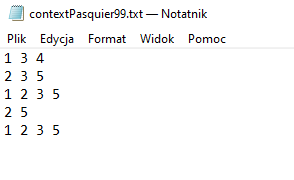
\includegraphics[scale=0.4]{DaneWejsciowe.png}
			\caption{Dane wejściowe}
		\end{figure}	
		
	\newpage
		
	\section{Wyniki}

		\begin{figure}[!h]
			\centering
			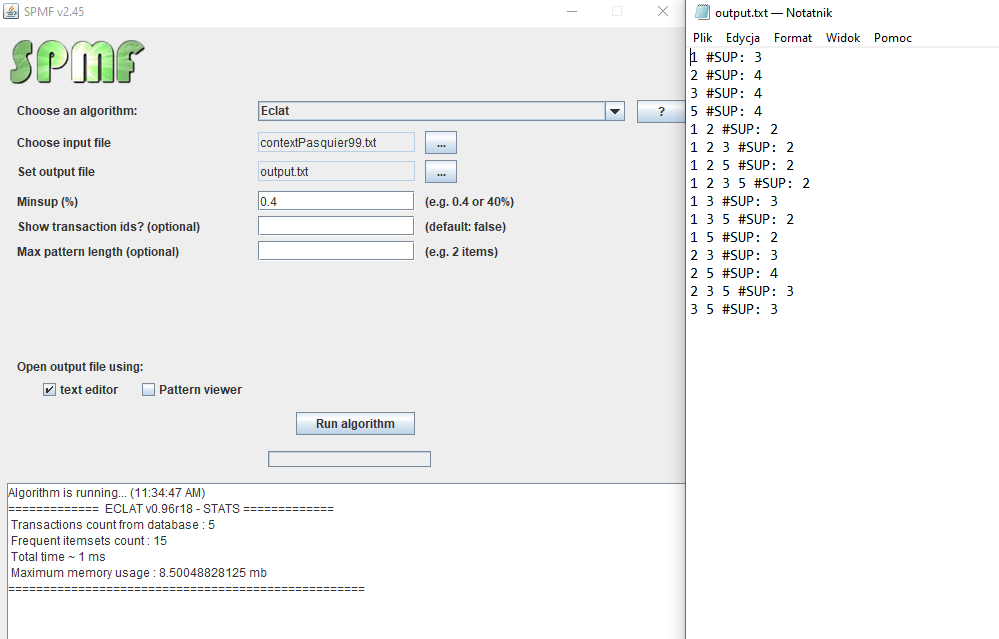
\includegraphics[scale=0.4]{Wejscie.png}
			\caption{Wyniki dzialania aplikacji}
		\end{figure}
		
	\section{Podsumowanie}

Algorytm Eclat posiada również istotne wady, główne narzuty związane z komunikacją wynikają z potrzeby ustalenia globalnych tid-list na początku algorytmu. W większości przypadków udaje się je zamortyzować w kolejnych iteracjach algorytmu. W trakcie wykonywania algorytmu dla różnych danych może dochodzić do nierównego obciążenia procesorów. Aby tego uniknąć liczba procesów powinna być dużo mniejsza niż liczba klas równoważności dla zbiorów częsty o długości 2. Aby osiągnąć dobrą wydajność algorytmu dla dowolnych danych może być konieczne przygotowanie strategii rodziału klas równoważności oraz równoważenie obciążeń.

	\section{Bibliografia}

Algorytm Eclat posiada również istotne wady, główne narzuty związane z komunikacją wynikają z potrzeby ustalenia globalnych tid-list na początku algorytmu. W większości przypadków udaje się je zamortyzować w kolejnych iteracjach algorytmu. W trakcie wykonywania algorytmu dla różnych danych może dochodzić do nierównego obciążenia procesorów. Aby tego uniknąć liczba procesów powinna być dużo mniejsza niż liczba klas równoważności dla zbiorów częsty o długości 2. Aby osiągnąć dobrą wydajność algorytmu dla dowolnych danych może być konieczne przygotowanie strategii rodziału klas równoważności oraz równoważenie obciążeń.
					
		
		
		\begin{enumerate}
			\item Nyćkowiak Jędrzej, Leśny Jacek (red.): Badania i Rozwój Młodych Naukowców w Polsce: Nauki techniczne i inżynieryjne. Cz. 2, 2019, Poznań, Młodzi Naukowcy, 196 s., ISBN 978-83-66392-43-4
			\item trójpasmowe z luminoforami wąskopasmowymi
			\item z luminoforami wielopasmowymi
		\end{enumerate} 	
	
	\clearpage % to mozna usunac w razie czego
	
\end{document}
